\chapter{Opis projektnog zadatka}
		
		\noindent CookBooked je projekt u kojem je potrebno razviti web aplikaciju koja omogućava korisnicima razmjenu recepata za kuhanje i pečenje kolača te povezivanje s autorima recepata. \\
		
		\noindent Neregistrirani korisnici mogu ssamo pregledavati recepte temeljem kategorija, vrsta kuhinje ili specifičnih sastojaka. Za pristup svim ostalim mogućnostima platforme, korisnici se moraju registrirati s važećom adresom e-pošte. \\
		
		\noindent Autori recepata imaju opciju komunikacije s ostalim korisnicima vezano za svoje recepte, kao npr. razmjenu poruka, čavrljanje ili video pozive. Ove značajke omogućuju korisnicima da se povežu s autorima recepata, ali su dostupne samo registriranim korisnicima. Autori recepata također mogu postaviti termine kada su dostupni za komunikaciju (npr. određene sate ili dane). \\
		
		\noindent Registrirano korisnici mogu označavati, komentirati i spremiti recepte za buduću referencu. Korisnici mogu pratiti svoje omiljene autore recepata kako bi primili obavijest o novim receptima.\\
		
		\noindent Registrirani korisnici imaju javne profile na kojima prikazuju svoje objavljene recepte, pratitelj i autore koje prate. Također imaju privatne profile gdje mogu upravljati osobnim informacijama, postavkama komunikacije i obavijestima za poruke i aktivnosti povezane s receptima. \\
		
		\noindent Platformu održavaju sistemski administratori koji mogu upravljati korisnicima, mijenjati kategorije recepata ili brisati recepte.
		
		
		
		\section{Opis ideje aplikacije}

		\noindent CookBooked je aplikacija koja omogućava korisnicima razmjenu recepata za kuhanje i pečenje kolača te povezivanje s autorima recepata. Sam potencijal ove aplikacije leži u dobro razvijenom te interaktivnom sučelju koje omogućava registriranim korisnicima lako objavljivanje svojih recepata, dok u isto vrijeme omogućava nesmetano korištenje i pregled samih tih recepata bez mogućnosti objave.\\
		
		\noindent Danas već postoje neke stranice za objavu recepata kao što su Coolinarka, ReciPeci, Zdrave navike i brojne druge. Iako su one već dobrim djelom razvijene te koriste brojne alate, aplikacija CookBooked omogućava veću personalizaciju, odabir jelovnika za pojedini dan te kategorizira jela i namirnice na načine koji su puno bliži i lakši za snalaženje svakom korisniku.\\

	
		\begin{figure}[H]
			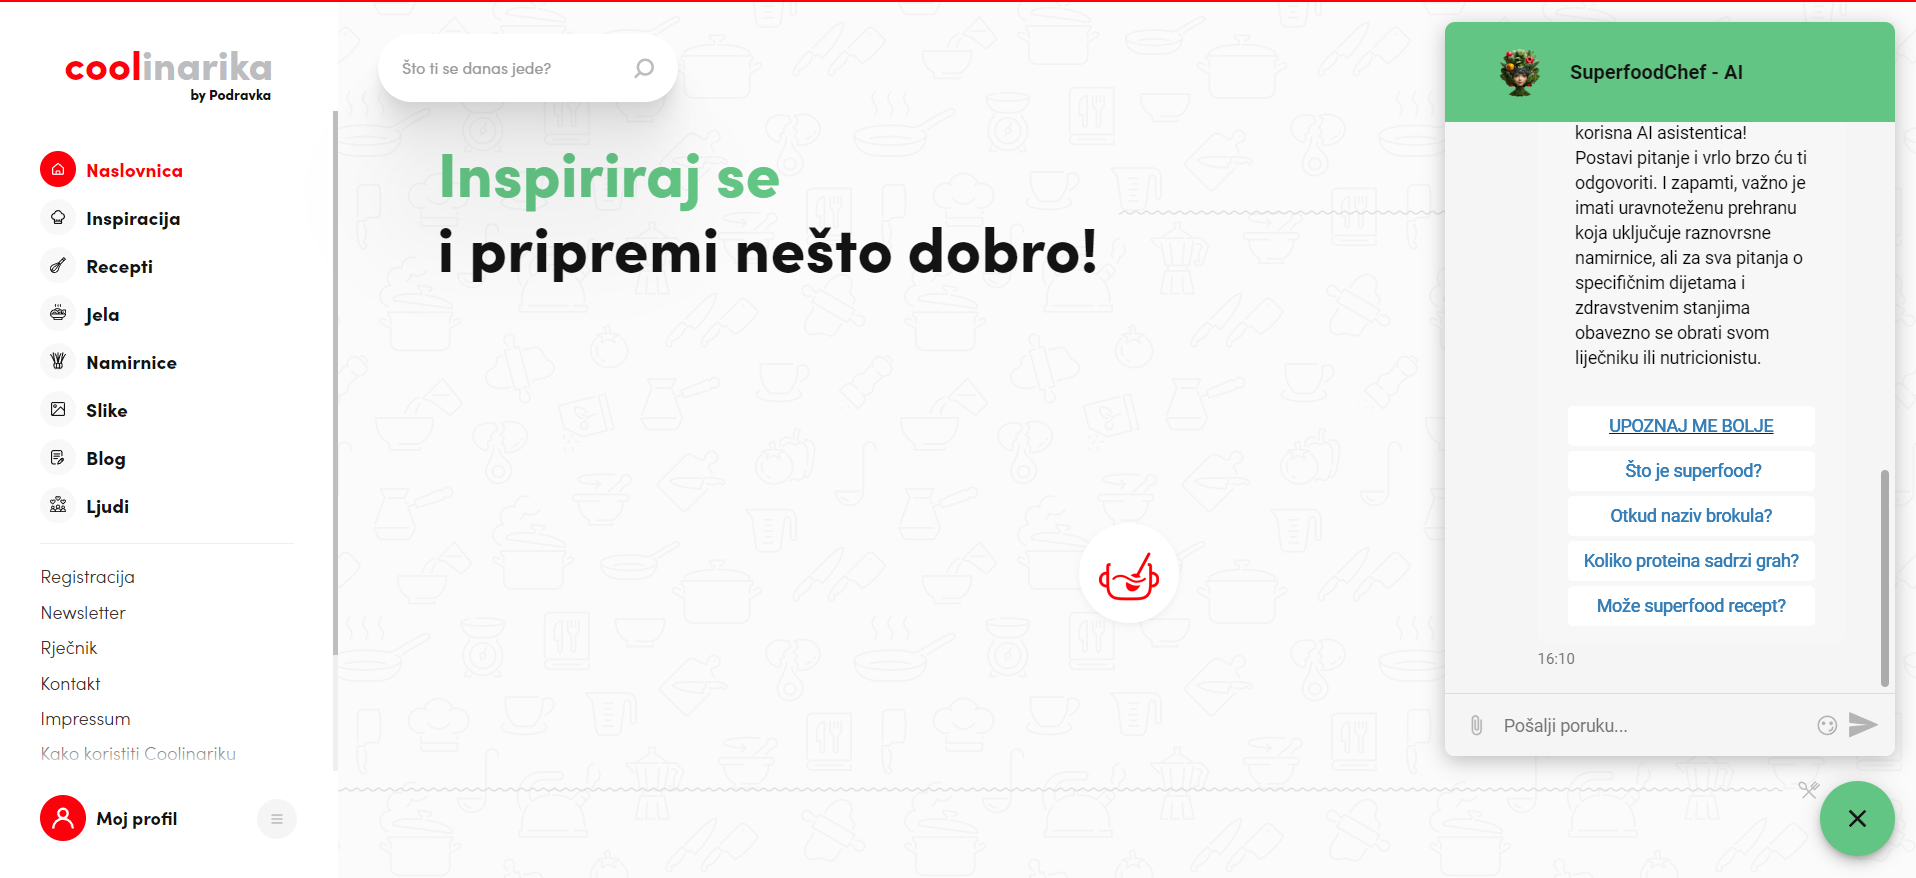
\includegraphics[scale= 0.3]{slike/coolinarka.png}
			\centering
			\caption{Coolinarka}
			\label{fig:Coolinarka}
		\end{figure} 
		
		\begin{figure}[H]
			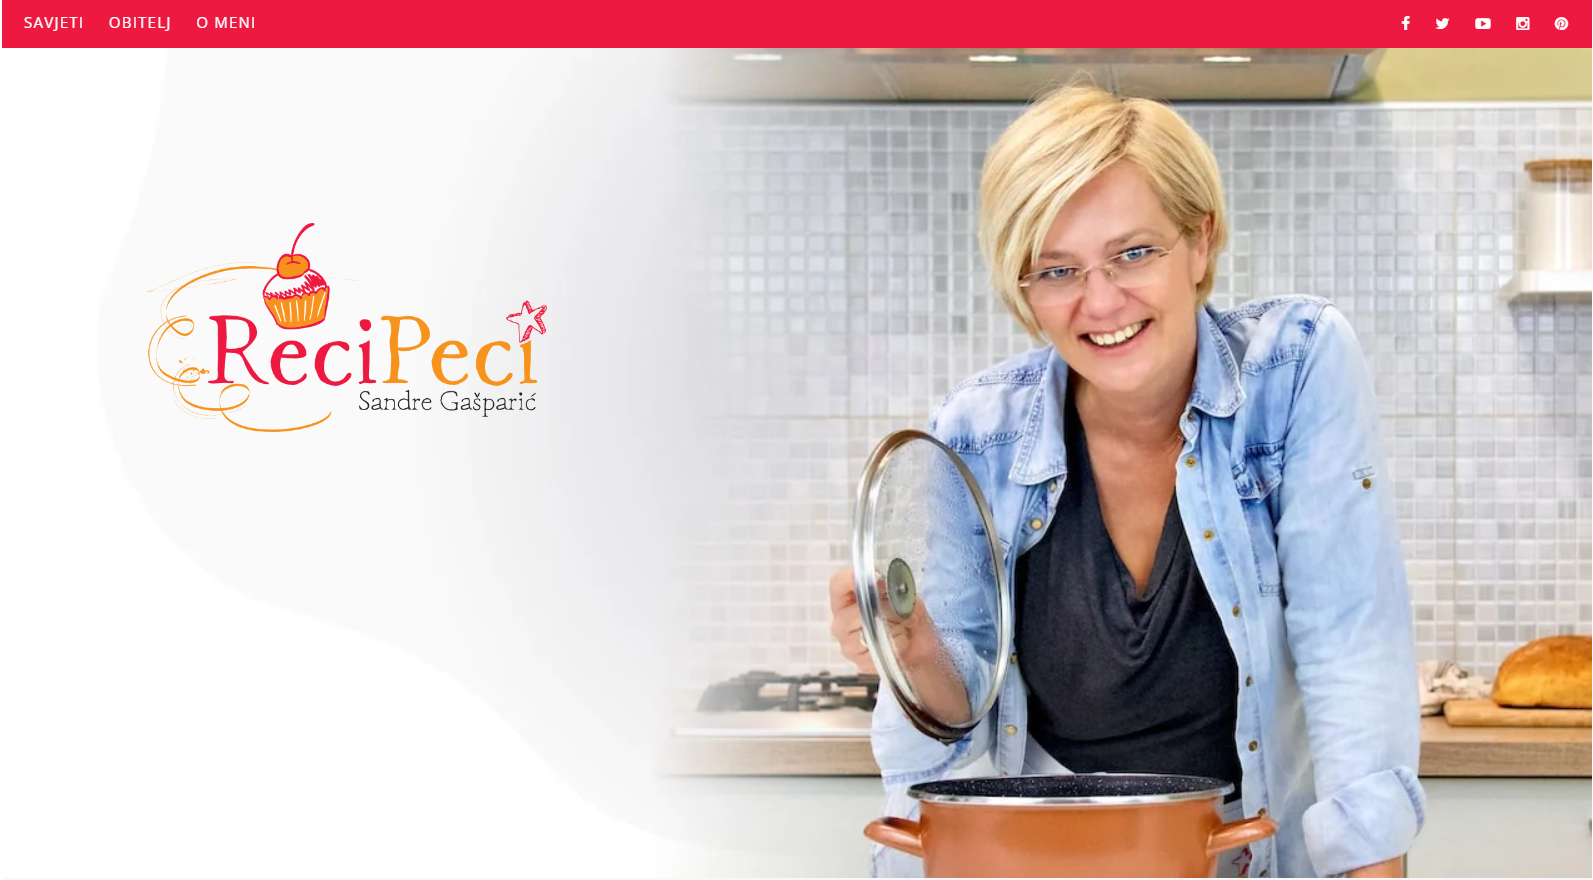
\includegraphics[scale= 0.3]{slike/recipeci.png}
			\centering
			\caption{ReciPeci}
			\label{fig:ReciPeci}
		\end{figure} 
		
		
		\noindent U prijašnjem odlomku spomenuli smo prednost odlične kategorizacije ove aplikacije pa tako gdje se ta prednost pokazuje jest upravo tako što imamo kategorije hrane za mlade, kategorije hrane za osobe sa bolestima te za starije osobe kojima odgovara lagana prehrana.\\
		
		\noindent Tako naša aplikacija zahvaća razne kategorije ljudi kao što su:
		\begin{packed_item}
			\item \textit{mlađe osobe koje tek uče kuhati}
			\item \textit{osobe koje ne stignu raditi duge pripreme}
			\item \textit{starije osobe koje ne mogu pripremati i konzumirati svu hranu}
			\item \textit{odrasli koji žele naučiti kuhati}
			\item \textit{osobe koje žele izraditi kompliciranije stvari sa nešto manje kulinarskog iskustva}
		\end{packed_item}
		
		\noindent Sama aplikacija od razvoja pa do konačne aplikacije i poslije je vrlo lako prilagodljiva. Osim izvornih alata pisanja koda, dijelove aplikacije lako je prilagoditi u smislu izgleda, dodavanja novih kategorija, dodatnih opcija privatnog profila. Ako želimo znati zašto, to je jednostavno. Cijela aplikacija u kodu je strukturirana na način da se prate i učitavaju određene strukture sa podatcima gdje je tada u slučaju bilo kakve modifikacije potrebno promjenu učiniti na samo jednom mjestu.\\
		
		\noindent Što se samih promjena tiče, aplikacija se sastoji od više verzija. Kod razvoja aplikacije u pogon se pušta prvo prototip koji sadrži osnovnu funkcionalnost zbog potrebe provjere ispravnosti aplikacije. U sljedećim verzijama aplikacija se nadograđuje profilima korisnika, poslovnim i privatnim profilima pa se nadalje dodaje i kategorije, izbornici, i slično te u konačnici mogućnost komunikacije između autora i recenzije njihovih recepata. \\
		
		\noindent Nakon završetka postavljenih ciljeva pri izradi aplikacije, zbog same strukture i čitljivosti pri pisanju, aplikaciju je u naknadnim verzijama moguće nadograditi sa brojnim drugim značajkama.\\
		Primjer takvih značajki:
		
		\begin{packed_item}
			\item \textit{komunikacija unutar aplikacije putem videopoziva}
			\item \textit{AI pomoć pri odabiru recepta i kategorije}
			\item \textit{AI stvaranje jelovnika prilagođenog za dan i posebne prilike}
			\item \textit{Stvaranje odjela za događaje izrade i objave novih recepata}
			\item \textit{Tečajevi za kuhanje putem videa i videopoziva}
		\end{packed_item}
		
	
		
		
		
		\eject
		
	